\section{Introduction}
\label{sec:intro}

Over the last decade, microcontrollers, the workhorses of embedded systems, have become
central to efforts in making~\cite{dougherty2012maker} and education. For example, the Arduino project
(\url{www.arduino.cc})~\cite{buildingArduino2014},
started in 2003, created the Uno board using an 8-bit Atmel
AVR microcontroller. The Uno makes its microcontroller's I/O pins available via headers;
external hardware modules (shields) may be connected to these headers to extend
the Uno's capability. The Arduino ecosystem has grown tremendously in the past 15 years,
with the support of companies, such as Adafruit Industries (\url{www.adafruit.com}) and
Sparkfun Electronics (\url{www.sparkfun.com}). that resell Arduino and make their
own Arduino-compatible boards. 

The Arduino platform has the following characteristics, common to many programming
environments for microcontrollers~\cite{XYZ}:
\begin{itemize}
\item it uses C/C++ as the starting programming language;
\item it loads code using 1980's era bootloader technology;
\item it encourages polling of sensors;
\item it lacks many interactive features of modern IDEs;
\end{itemize}
These characteristics make such systems non-trivial for beginners to work with, 
require the installation of OS-specific drivers/applications/toolchains,
and leads to poor programming practices.

The Java language (among others) held out the promise of a better way forward for 
programming microcontrollers, but XYZ.  
\flameon{we need more description of why current ways of programming microcontrollers 
make for a high barrier to entry; also need to take on Java head on here, as well as
RTOS and MicroPython.}

In contrast to the situation for programming microcontrollers, 
on the web we find many excellent environments for introductory programming.
Visual block editors such as Scratch (\url{https://scratch.mit.edu/})~\cite{ScratchCACM2009,BlocksBeyondCACM2017}
and Blockly (\url{https://developers.google.com/blockly/})~\cite{Blocky2015}
allow the creation of programs without the possibility of syntax errors.
The programming models associated with Scratch and Blockly generally are
event based, freeing the programmer from the need to poll.
HTML, CSS and JavaScript allow a complete programming experience to be delivered as an interactive
web app, including editing with intellisense, code execution and debugging~\cite{Monaco}. 

With a surge in the demand of microcontroller-based devices for education~\cite{XYZ}, 
there is a need to simplify the programming of such devices so that they suitable 
for novice users in restricted environments.
Therefore, we have created a new programming platform that bridges the worlds of 
the microcontroller and the web app. 

The major goals of the platform are to:
% TypeScript / Blocks + MakeCode
(1) make it simple to program microcontrollers in a higher-level language,
using nothing more than a web app;
% TypeScript and Blocks prevent users from making boo boos.
(2) provide a safe environment for users to develop programs for microcontrollers;
% simulator, auto completion...
(3) create a feature rich and extensible development environment that decreases time taken to program a microcontroller (time to awesome);
% UF2 is awesome
(4) allow a users' compiled program to be easily installed on a microcontroller;


The platform consists of a stack of four novel technologies, the subject of
this paper:
\begin{itemize}
\item \emph{\MC (\href{https://makecode.com}{makecode.com})}, a web app that supports both visual block programming and text programming,
via \emph{Static TypeScript}, with conversion between the two program representations (Section~\ref{sec:makecode});

\item \emph{Static TypeScript}, a statically-typed subset of TypeScript (\url{www.typescriptlang.org}),
a gradually-typed superset of JavaScript, for fast execution on low-memory devices, with
a simple model for linking against pre-compiled C++ (Section~\ref{sec:sts});

\item \emph{\CO (the Component-oriented Device Abstraction Layer)}, an event driven, multi-threaded, C++ runtime environment that bridges the semantic gap between higher-level languages and the hardware,
modelling each hardware component as a software component (Section~\ref{sec:codal});

\item \emph{USB Flashing Format} (UF2), a new file format designed for flashing microcontrollers 
over the Mass Storage Class protocol (USB pen drives); the format greatly speeds the installation of user
programs and is robust to differences in operating systems (Section~\ref{sec:uf2}).
\end{itemize}
The \MC web app is the entry point of the platform, and has in-browser execution via a device simulator, as well as compilation to machine code and linking against a
pre-compiled C++ runtime (\emph{\CON}). No C/C++ compiler is invoked to compile user code and the result of compilation is a binary file that is ``downloaded'' from the web app to the user's
computer and then flashed to the microcontroller (exposed as a USB pen drive) 
via a simple file copy operation,  with the aid of the \emph{UF2} file format and supporting firmware. 


\begin{figure*}[t]
      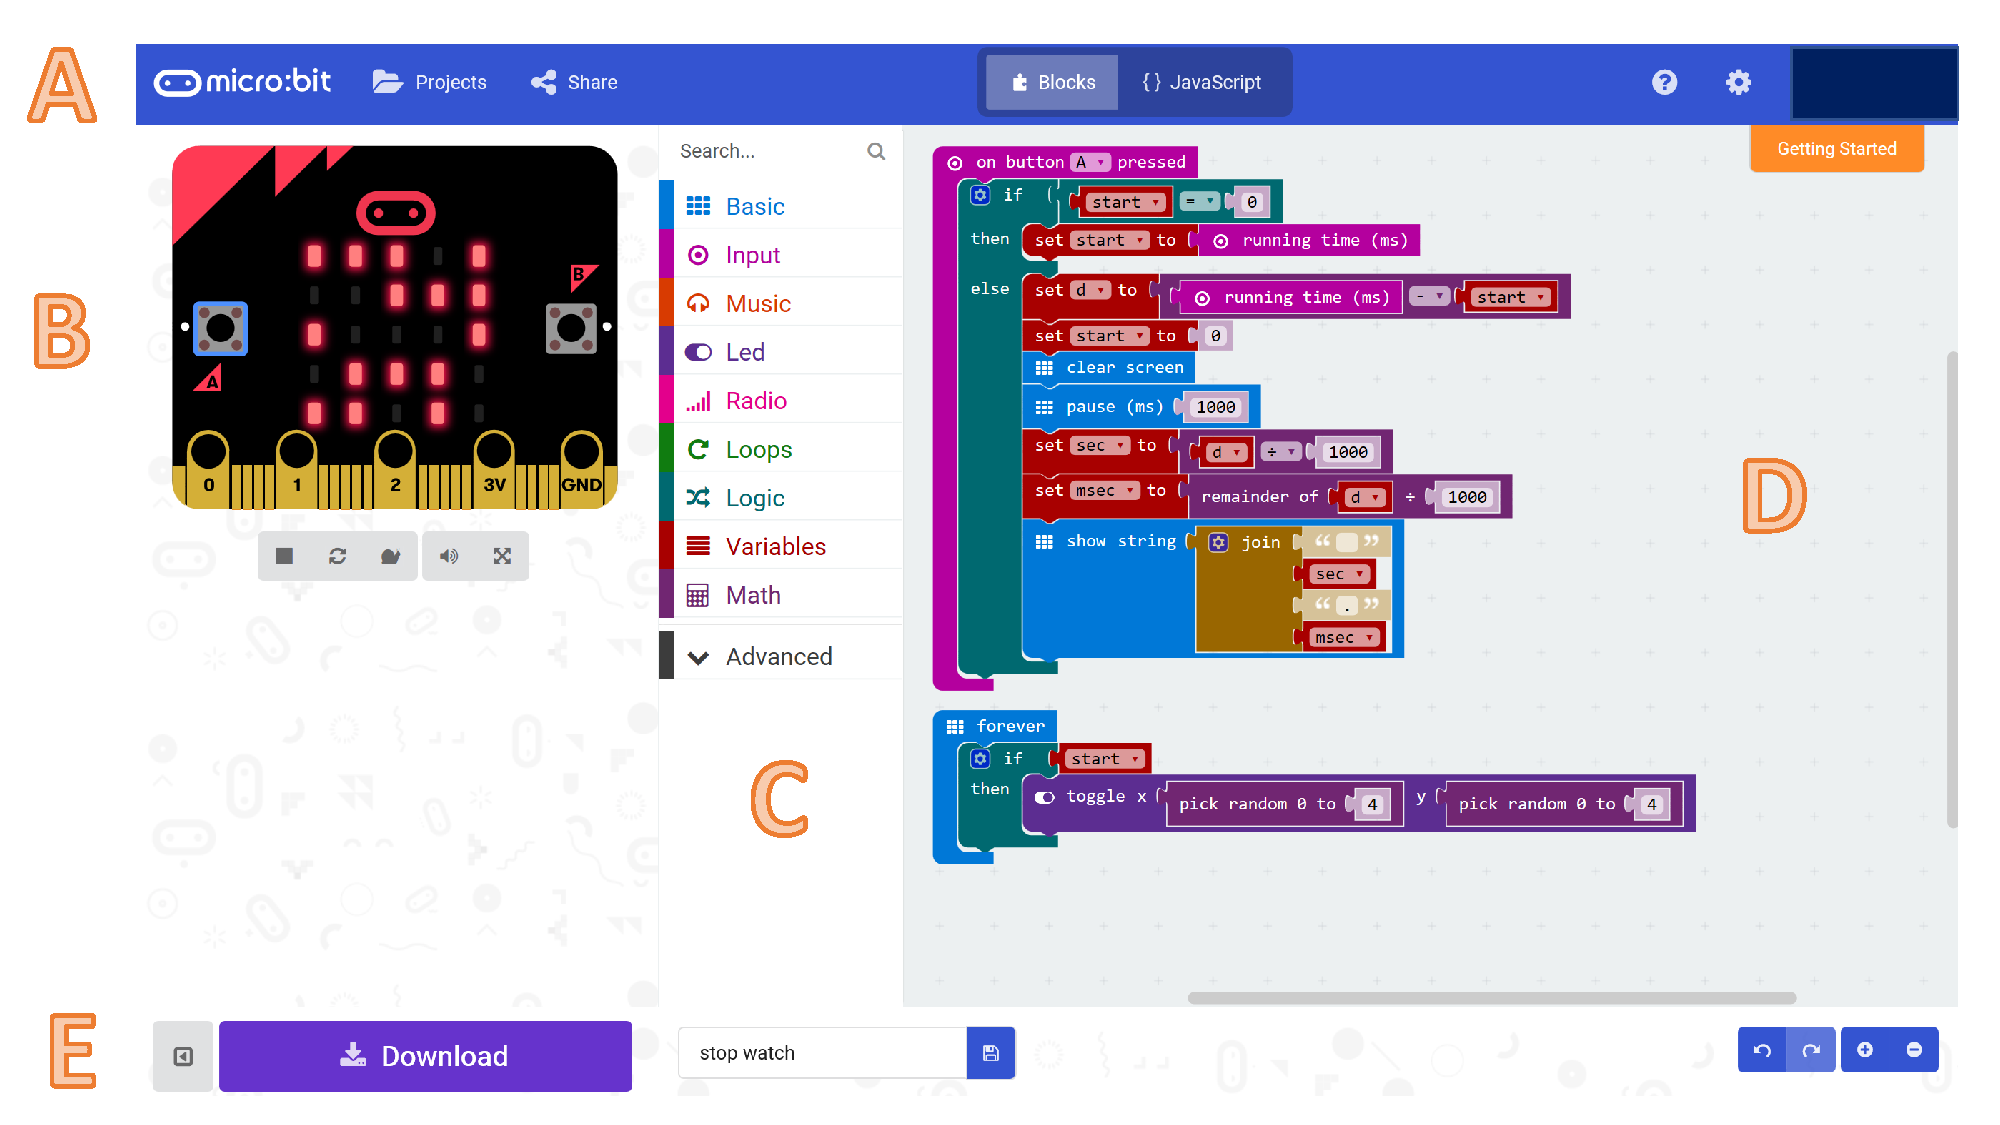
\includegraphics[width=5in]{screenSnapFig.pdf}
  \caption{\label{fig:screenSnap}Screen snapshot of the \MC web app. \flameon{TODO:remove the MSFT logo}}
  \end{figure*}


These four advances enable beginners to get started programming microcontrollers from any modern web browser, and enable
hardware vendors to innovate and safely add new components to the mix using Static TypeScript, leveraging its
foreign function interface to C++.
Once the web app has been loaded, all the above functionality works offline (i.e., if the host machine loses its connection
to the internet).

\begin{table}[]
\centering
\begin{tabular}{|l|l|l|l|l|}
\hline
Device             & RAM (kB) & Flash (kB) & Word Size        \\ \hline
Arduino Uno        & 2        & 32         & 8               \\ \hline
BBC micro:bit      & 16       & 256        & 32              \\ \hline
Circuit Playground & 32       & 256        & 32              \\ \hline
\end{tabular}
\caption{\label{table:devices}A subset of devices supported by the platform.}
\end{table}
Whilst this paper focuses on three devices listed in Table~\ref{table:devices}, we encourage the reader to choose a target
from \url{www.makecode.com} and experiment with programming it, to appreciate the
qualitative aspects of the platform, namely its simplicity and ease of use.
This paper evaluates quantitative aspects of the platform:
compilation speed, code size, and runtime performance.  In particular, we
consider:
\begin{itemize}
\item the time to compile Static TypeScript user code (to machine code) with respect
      to the GCC C/C++ toolchain, as well as the size of the resulting executable;
\item the time to load code onto a microcontroller using UF2, compared to standard bootloaders
      such as Arduino and ARM's DAPlink;
\item the performance of a set of small benchmarks, written in both Static TypeScript and C++,
      compiled with the \MC and GCC toolchains;
\item \emph{energy consumption: \CO vs. Arduino}
\item \emph{native code vs. bytecode} we
      evaluate memory consumption and code performance for native code generation
      vs. bytecode generation and interpretation on the Uno.
\end{itemize}

\flameon{TODO: we should present some of high-level experimental results here.}

All of the platform's components are open source on GitHub.
  
Sections~\ref{sec:makecode} to~\ref{sec:uf2} presents the four major components of the platform, top-down,
as referenced before. Section~\ref{sec:evaluate} evaluates the performance of the platform,
Section~\ref{sec:related} discusses related work, and Section~\ref{sec:conclude}
concludes.
